% Copyright (C) 2012 Raniere Silva
%
% This work is licensed under the Creative Commons
% Attribution-ShareAlike 3.0 Unported License. To view a copy of this
% license, visit <http://creativecommons.org/licenses/by-sa/3.0/>.
%
% This work is distributed in the hope that it will be useful, but
% WITHOUT ANY WARRANTY; without even the implied warranty of
% MERCHANTABILITY or FITNESS FOR A PARTICULAR PURPOSE.

\documentclass[11pt]{beamer}

\usetheme{CambridgeUS}
\let\Tiny=\tiny % Redefine at least \Tiny for avoid warning

\usepackage[utf8]{inputenc}
\usepackage[T1]{fontenc}

\usepackage[brazil]{babel}
\usepackage{indentfirst}
\uselanguage{brazil}
\languagepath{brazil}
\deftranslation[to=brazil]{Example}{Exemplo}

\usepackage{url}
\usepackage{hyperref}
\usepackage{breakurl}

\usepackage{xmpincl}

\usepackage{amsmath}
\usepackage{amsfonts}
\usepackage{amssymb}
\usepackage{amsthm}
\usepackage{breqn}

\usepackage{multicol}
\usepackage{multirow}
\usepackage{array}

\usepackage{graphicx}
\usepackage{subfigure}
\usepackage{wrapfig}
\usepackage{tikz}

\usepackage{algorithmic}
\algsetup{linenosize=\small}

\usepackage{algorithm}
\floatname{algorithm}{Algoritmo}

\usepackage{textcomp}
\usepackage{listings}
\lstset{
% language=Octave,
basicstyle=\ttfamily\scriptsize,
columns=flexible,
% numbers=left,
% numberstyle=\footnotesize,
% stepnumber=5,
% numbersep=5pt,
% backgroundcolor=\color{white},
% showspaces=false,
% showstringspaces=false,
% showtabs=false,
% frame=single,
tabsize=4,
captionpos=t,
breaklines=true,
breakatwhitespace=false,
% caption={\texttt{\lstname}},
% escapeinside={\%*}{*)},
% morekeywords={#},
upquote=true,
}

% Index
\usepackage{makeidx}
\makeindex


\newcommand{\flang}[1]{\textit{#1}}

\hypersetup{
pdftitle={EPUB3: O livro no século 21},
pdfauthor={Raniere Silva},
pdfsubject={EPUB3, ebook, livro digita, livro eletrônico, padrões abertos},
pdfcreator={Raniere Silva},
pdfkeywords={EPUB3, ebook, livro digita, livro eletrônico, padrões abertos}
}
\includexmp{epub_20th}

\newtheorem{defi}{Definição}
\newtheorem{prop}{Proposição}

\renewcommand{\algorithmicrequire}{\textbf{Entrada:}}
\renewcommand{\algorithmicensure}{\textbf{Saída:}}
\renewcommand{\algorithmicend}{\textbf{fim}}
\renewcommand{\algorithmicif}{\textbf{se}}
\renewcommand{\algorithmicthen}{\textbf{ent\~{a}o}}
\renewcommand{\algorithmicelse}{\textbf{caso contr\'{a}rio}}
\renewcommand{\algorithmicendif}{\algorithmicend}
\renewcommand{\algorithmicfor}{\textbf{para}}
\renewcommand{\algorithmicforall}{\textbf{para todo}}
\renewcommand{\algorithmicdo}{\textbf{fa\c{c}a}}
\renewcommand{\algorithmicendfor}{\algorithmicend}
\renewcommand{\algorithmicwhile}{\textbf{enquanto}}
\renewcommand{\algorithmicendwhile}{\algorithmicend}
\renewcommand{\algorithmicrepeat}{\textbf{repita}}
\renewcommand{\algorithmicuntil}{\textbf{at\'{e}}}
\renewcommand{\algorithmicreturn}{\textbf{retorne}}
\renewcommand{\algorithmiccomment}[1]{\hspace{2em}/* #1 */}

\renewcommand{\lstlistingname}{C\'{o}digo}

\begin{document}
\title[EPUB3]{EPUB3: O livro no século 21}
\author[Raniere Silva]{Raniere Gaia Costa da
Silva\footnote{ra092767@ime.unicamp.br}}
\date{27/03/2013}

\begin{frame}
  \maketitle
\end{frame}

\begin{frame}
  \begin{block}{}
    Os arquivos desta apresentação encontram-se disponíveis \\
    em \url{https://github.com/r-gaia-cs/presentations}. \\
    \vspace{-33pt}
    \begin{flushright}
      \includegraphics[height=2cm]{../figures/forkme_right_red.png}
    \end{flushright}
  \end{block}

  \begin{block}{Licença}
    Salvo indicado o contrário, esta apresentação está licenciada sob a
    Licença Creative Commons Atribuição-CompartilhaIgual 3.0 Não Adaptada.
    Para ver uma cópia desta licença, visite
    \url{http://creativecommons.org/licenses/by-sa/3.0/deep.pt_BR}.
    \begin{center}
      
\includegraphics{../figures/cc-by-sa.png}
    \end{center}
  \end{block}
\end{frame}

% \begin{frame}{Sobre o que é essa palestra}
%   \begin{itemize}
%     \item Padrões abertos,
%     \item EPUB3 (\flang{electronic publication version 3}),
%     \item DRM (\flang{Digital rights management}).
%   \end{itemize}
% \end{frame}

\begin{frame}{Sobre o que não é essa palestra}
  \begin{itemize}
    \item \flang{ereaders} (e.g., Kobo, Kindle, \ldots),
    \item \flang{tablets},
    \item lojas de livros digitais.
  \end{itemize}
\end{frame}

\begin{frame}
    \tableofcontents
\end{frame}

\section{Contesto histórico}
\begin{frame}
  \begin{columns}
    \begin{column}[t]{.4\textwidth}
      \begin{itemize}
        \item 1995-1999:
          \pause
          \begin{itemize}
            \item Popularição da Web.
              \pause
            \item Primeiros tocadores de mp3.
              \pause
            \item Lançamento do Napster (Junho de 1999).
              \pause
          \end{itemize}
        \item 2000-2005:
          \pause
          \begin{itemize}
            \item Lançamento do iPod (Novembro de 2001).
              \pause
            \item Lançamento do iTunes (Abril de 2003).
              \pause
          \end{itemize}
      \end{itemize}
    \end{column}
    \begin{column}[t]{.4\textwidth}
      \begin{itemize}
        \item 2005-2009:
          \pause
          \begin{itemize}
            \item Primeiros modelos de \flang{ereaders}.
              \pause
            \item Lançamento do Kindle (Novembro de 2007).
              \pause
          \end{itemize}
          \item 2010-hoje
            \pause
            \begin{itemize}
              \item Lançamento do iPad (Março de 2010).
            \end{itemize}
        \end{itemize}
    \end{column}
  \end{columns}
\end{frame}

\section{EPUB3}
\nocite{ebookFormat}
\begin{frame}{Outros formatos}
  \begin{itemize}
    \item PostScript (.ps);
      \pause
    \item Adobe Portable Document Format (.pdf);
      \pause
    \item DjVu (.djvu);
      \pause
    \item Mobipocket (.mobi);
      \pause
    \item KF8 (.azw; .kf8);
      \pause
    \item iBook (.ibooks);
%     \pause
%   \item Comic Book Archive file (.cbz);
  \end{itemize}
\end{frame}

\begin{frame}{Responsabilidade}
  \flang{International Digital Publishing Forum}
\end{frame}

\begin{frame}{Macro estrutura}
  \begin{center}
    \only<1>{
\includegraphics[width=.4\textwidth]{../figures/epub_logo.png}}
    \only<2>{
\includegraphics[width=.4\textwidth]{../figures/zip_blue_logo.png}}
    \only<3>{
\includegraphics[width=.4\textwidth]{../figures/xml_file_logo.png}}
  \end{center}
\end{frame}

\begin{frame}{Micro estrutura}
  \begin{center}
    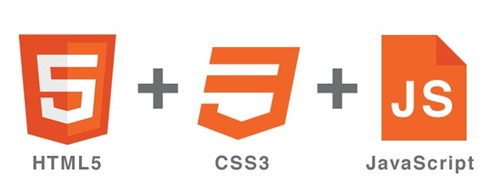
\includegraphics[width=.8\textwidth]{../figures/html5-css3-javascript.jpg}
  \end{center}
\end{frame}

\section{Mudanças do EPUB2 para EPUB3}
\nocite{epub3Changes}
\begin{frame}{Conteúdo}
  \begin{itemize}
    \item HTML5 \pause(Incluindo audio e vídeo)
      \pause
    \item SVG
      \pause
    \item MathML
      \pause
    \item Javascript
  \end{itemize}
\end{frame}

\begin{frame}{\flang{Layout}}
  \begin{itemize}
    \item Fluído
      \pause
    \item CSS(3)
      \pause
    \item Fontes
      \pause
    \item \flang{Overlay}
  \end{itemize}
\end{frame}

%\section{Readium}
%\begin{frame}{Leitor e SDK}
%  Readium
%\end{frame}

\section{DRM}
\begin{frame}{O que é?}
  \flang{Digital rights management} é uma tecnologia de controle de acesso
  utilizada com a intenção de limitar o uso de conteúdo digital depois da venda.
\end{frame}

\begin{frame}{Como funciona}
  \begin{center}
    \begin{tikzpicture}
      \node (l) at (0,0) {loja};
      \node (r) at (0,-4) {leitor};

      \draw[->] (l) -- (r);
    \end{tikzpicture}
    \hspace{.25\textwidth}\pause
    \begin{tikzpicture}
      \node (l) at (0,0) {loja};
      \node (d) at (0,-2) {equip.};
      \node (r) at (0,-4) {leitor};

      \draw[->] (l) -- (d) node[midway, right] {encriptar};
      \draw[->] (d) -- (r) node[midway, right] {desencriptar};
    \end{tikzpicture}
  \end{center}
\end{frame}

\begin{frame}{Controvérsias}
  O uso de DRM envolve alguns questionamentos relacionados com a propriedade
  física e o direito autoral.
\end{frame}

\section*{Obrigado}
\begin{frame}
  \begin{center}
    Obrigado!
  \end{center}
  \begin{center}
    \url{r.gaia.cs@gmail.com}
  \end{center}
\end{frame}

\section*{Bibliografia}
\begin{frame}
  \bibliography{epub_20th}
  \bibliographystyle{alpha}
\end{frame}
\end{document}
